\chapter{Foundations: Data Systems}
\label{chap:data-systems}

\section{The central idea}
\label{sec:data-systems-central-idea}

A data system is mostly a set of decisions about where data lives, how it is represented, and how you expect to access it.

An \textbf{Access Pattern} can be thought of as a systems inductive bias.
\begin{itemize}
    \item CNN: locality
    \item Transformer: interactions should be learnable through attention
    \item Redis assumes that the key$\rightarrow$value is the limiting operation
    \item columnar format assumes we read a few columns across many rows
    \item vector database assumes that nearby embeddings represent semantically similar items
\end{itemize}

Understanding the \textbf{bias} usually tells you when to use the system.

\section{Overview}
\label{sec:data-systems-overview}

\begin{figure}[htbp]
\centering
\resizebox{0.98\linewidth}{!}{%
\begin{tikzpicture}[
  >=Latex,
  node distance=7mm and 13mm,
  box/.style={draw, rounded corners, align=center, minimum width=31mm, minimum height=10mm, inner sep=4pt},
  smallbox/.style={draw, rounded corners, align=center, minimum width=29mm, minimum height=9mm, inner sep=3pt},
  arrow/.style={->, thick},
  note/.style={align=left, font=\small}
]
\node[align=center,box] (object) {Object store\\S3 / GCS};
\node[align=center,box, below=of object] (ssd) {Local SSD\\cache};
\node[align=center,box, below=of ssd] (ram) {RAM\\DataLoader};
\node[box, below=of ram] (gpu) {GPU memory};

\draw[arrow] (object) -- node[right, note]{Parquet / shards / files} (ssd);
\draw[arrow] (ssd) -- (ram);
\draw[arrow] (ram) -- node[right, note]{batch} (gpu);

\node[smallbox, right=28mm of object] (pg) {Postgres};
\node[align=center,note, right=4mm of pg] {experiment metadata\\users / labels / jobs};

\node[smallbox, right=28mm of ssd] (redis) {Redis};
\node[align=center,note, right=4mm of redis] {fast cache\\temporary state};

\node[smallbox, right=28mm of ram] (vector) {Vector DB};
\node[note, right=4mm of vector] {embedding retrieval};

\node[smallbox, right=28mm of gpu] (kafka) {Kafka-like log};
\node[note, right=4mm of kafka] {streams of events};

\node[align=center, font=\bfseries, above=5mm of object] {DURABLE / LARGE / CHEAP};
\node[align=center, font=\bfseries, below=5mm of gpu] {FAST / SMALL / EXPENSIVE};
\end{tikzpicture}%
}
\caption{A useful first mental model for an ML data system. Data moves from durable, large storage toward progressively faster and smaller memory as computation approaches the GPU. Other stores serve different access patterns rather than forming one single hierarchy.}
\label{fig:data-systems-master-picture}
\end{figure}


\begin{table}[htbp]
\centering
\caption{The recurring questions to ask about every storage or data-system component. 
You should be able to look at each arrow in Figure \ref{fig:data-systems-master-picture} and ask what the requirements are, based on Table \ref{tab:data-systems-six-questions}.
}
\label{tab:data-systems-six-questions}
\begin{tabularx}{\linewidth}{@{}lX@{}}
\toprule
\textbf{Property} & \textbf{Question} \\
\midrule
Capacity & How much data can this layer hold economically? \\
Latency & How long does one access take before useful data begins arriving? \\
Bandwidth & How much data can move per second once transfer is underway? \\
Cost & What do storage, memory, compute, and network traffic cost? \\
Durability & What happens to the data after crashes or machine loss? \\
Access pattern & Exact lookup, range query, scan, stream, similarity search, or sequential read? \\
\bottomrule
\end{tabularx}
\end{table}

\clearpage
\section{Data structures}
\label{sec:data-structures}

\subsection{Arrays and Tensors}
\label{subsec:arrays-native-language}
An array is conceptually a structured set of filled memory dimensions. 
The important property is that elements are laid out predictably in memory.
\begin{verbatim}
memory: [3.2][1.7][8.1][0.4][2.9]
\end{verbatim}

A tensor is essentially:
\begin{verbatim}
array:
    shape
    dtype
    strides
    device
\end{verbatim}

For example,$\overbrace{X}^{\text{tensor}} \in
\mathbb{R}^{\overbrace{32}^{\text{images}}
\times \overbrace{3}^{\text{channels}}
\times \overbrace{224}^{\text{height}}
\times \overbrace{224}^{\text{width}}}$
might mean 32 images, 3 channels, 224 pixels, 224 pixels.

\paragraph{Efficiency}
Suppose the CPU asks for \verb|X[100]|.
The address can essentially be calculated directly without a costly search operation.
This gives approximately constant-time random access.
\[
\underbrace{a_{100}}_{\text{address of element 100}}
=
\underbrace{a_0}_{\text{base address}}
+
\underbrace{100}_{\text{index}}
\times
\underbrace{s}_{\text{bytes per element}}.
\]


\paragraph{Memory locality}

Processors rarely fetch exactly one number.
They fetch blocks of nearby memory into caches.
So reading
\begin{verbatim}
X[0],X[1],X[2],X[3]
\end{verbatim}
is generally much friendlier than
\begin{verbatim}
X[2],X[92817],X[71],X[831]
\end{verbatim}
This is \textbf{locality}, and is often why \textbf{contiguous} data is valued higher than non-contiguous data.

\paragraph{Strides}
Suppose matrix
\[
    X=
    \begin{bmatrix}
    a & b & c\\
    d & e & f
    \end{bmatrix}
\]
with memory \textsc{[a][b][c][d][e][f]}.
The tensor can walk through the same memory using different strides without rearranging the memory.
That is why PyTorch sometimes complains that something is \textbf{non-contiguous}.

\begin{calloutpracticaltip}
    When you see \verb|x.contiguous()|, the system may be making a new copy whose memory layout is easier for the next operation to consume.
\end{calloutpracticaltip}

\subsection{Hash Maps}
\label{subsec:hash-maps}

Python code such as
\begin{verbatim}
    cache["user_172"] = embedding
\end{verbatim}
is based conceptually on a hash table.

\begin{figure}[htbp]
    \centering
    \begin{tikzpicture}[>=Latex, node distance=13mm, every node/.style={align=center}]
    \node[draw, rounded corners, minimum width=28mm, minimum height=9mm] (key) {\texttt{"user\_172"}};
    \node[draw, rounded corners, right=of key, minimum width=28mm, minimum height=9mm] (hash) {hash function};
    \node[draw, rounded corners, right=of hash, minimum width=25mm, minimum height=9mm] (bucket) {bucket 431};
    \node[draw, rounded corners, right=of bucket, minimum width=28mm, minimum height=9mm] (value) {embedding};
    \draw[->, thick] (key) -- (hash);
    \draw[->, thick] (hash) -- (bucket);
    \draw[->, thick] (bucket) -- (value);
    \end{tikzpicture}
    \caption{Conceptual hash-table lookup.}
    \label{fig:hash-map-flow}
\end{figure}

The goal is approximately
\[
    \underbrace{T_{\text{lookup}}}_{\text{lookup time}}
    \approx
    \underbrace{O(1)}_{\approx \text{independent of table size}}.
\]

Meaning the lookup does not normally become much slower just because you have millions of entries.

\textbf{Collision} may occur when two keys map to the same hash.


\begin{calloutintuition}
    Hash maps trade ordering for extremely fast exact lookup.
\end{calloutintuition}

A hash map assumes that you know the key exactly

\subsection{Trees: fast ordered lookup}
\label{subsec:trees-ordered-lookup}
Imagine sorted values:
\begin{center}
    \begin{tikzpicture}[level distance=10mm, level 1/.style={sibling distance=40mm}, level 2/.style={sibling distance=20mm}, every node/.style={circle, draw, minimum size=7mm}, edge from parent/.style={draw,-Latex}]
    \node {50}
     child {node {20}
       child {node {5}}
       child {node {35}}
     }
     child {node {80}
       child {node {65}}
       child {node {95}}
     };
    \end{tikzpicture}
\end{center}
You eliminate large parts of the search space each step.
\[
    \underbrace{T_{\text{tree lookup}}}_{\text{lookup work}}
    \propto
    \log n
\]

% BOOK-LINK: If the tree-based models chapter discusses trees, explicitly distinguish
% algorithmic search trees from decision trees. The shared object is the recursive
% partitioning structure; the purpose is different.

\subsubsection{B-trees / B+ trees}
Binary trees are not ideal for disks because disk/database systems read data in blocks called \textbf{pages} and so databases usually prefer very wide trees.
\begin{center}
\begin{tikzpicture}[>=Latex, node distance=7mm and 8mm]
\node[draw, rounded corners, minimum width=28mm] (root) {root page};
\foreach \x/\name in {-4/p1,-2/p2,0/p3,2/p4,4/p5} {
  \node[draw, rounded corners, below=16mm of root, xshift=\x cm, minimum width=19mm] (\name) {page};
  \draw[->] (root) -- (\name);
}
\end{tikzpicture}
\end{center}

One page can contain many keys.
That reduces the number of storage accesses required.



\begin{calloutpracticaltip}
    A hash index is excellent for exact lookup.
    A tree index is excellent for ordered/range lookup.
\end{calloutpracticaltip}


\subsection{Queues}
\label{subsec:queues}

Suppose your CPU prepares training batches faster or slower than your GPU consumes them - the queue between them acts as a buffer.

\begin{figure}[htbp]
    \centering
    \begin{tikzpicture}[>=Latex, node distance=12mm]
    \node[draw, rounded corners, minimum width=28mm, minimum height=9mm] (cpu) {CPU workers};
    \node[draw, rounded corners, right=of cpu, minimum width=45mm, minimum height=13mm] (queue) {batch 1 \quad batch 2 \quad batch 3};
    \node[draw, rounded corners, right=of queue, minimum width=22mm, minimum height=9mm] (gpu) {GPU};
    \draw[->, thick] (cpu) -- (queue);
    \draw[->, thick] (queue) -- (gpu);
    \end{tikzpicture}
    \caption{A queue buffers work between a producer and a consumer.}
    \label{fig:producer-consumer-queue}
    \end{figure}
    Examples include:
    \begin{verbatim}
    DataLoader -> batch queue -> GPU
    web app -> job queue -> GPU inference worker
    event generator -> Kafka -> data pipeline
\end{verbatim}

The producer and consumer can run at different speeds, which is extremely useful. 

\paragraph{Backpressure}

Suppose rates $r_{\text{producer}} \gg r_{\text{consumer}}$, the queue grows by the difference.
Eventually a fix is needed, by: slowing producer, dropping data, increaseing  consumers, increasing buffering, fail
This is \textbf{backpressure}.
You will encounter this idea everywhere in distributed ML systems.

\subsection{Graphs and DAGs}
\label{subsec:graphs-dags}

A graph is a set of objects connected by relationships.
In ML systems, a particularly important version is a \textbf{directed acyclic graph} (DAG):

\begin{figure}[htbp]
\centering
\begin{tikzpicture}[>=Latex, node distance=10mm and 22mm, every node/.style={draw, rounded corners, align=center, minimum width=25mm, minimum height=8mm}]
\node (raw) {raw data};
\node[below=of raw] (clean) {clean};
\node[below left=of clean] (train) {train};
\node[below right=of clean] (val) {validation};
\node[below=of train] (model) {model};
\draw[->] (raw) -- (clean);
\draw[->] (clean) -- (train);
\draw[->] (clean) -- (val);
\draw[->] (train) -- (model);
\end{tikzpicture}
\caption{A DAG represents dependencies in a data or experiment pipeline.}
\label{fig:data-pipeline-dag}
\end{figure}

DAGs represent dependencies, from which workflow managers can say \textit{Step C cannot run until A and B are complete}.
You already implicitly use graphs when thinking about computational graphs, neural networks, data pipelines, and experiment dependencies.

% BOOK-LINK: Link this DAG discussion to the neural-network computational-graph section.

\section{Storage Hierarchy}
\label{sec:storage-hierarchy}

A computer has multiple storage levels.

\begin{figure}[htbp]
\centering
\begin{tikzpicture}[node distance=2mm, every node/.style={draw, minimum height=7mm, align=center}]
\node[minimum width=32mm] (reg) {CPU registers};
\node[below=of reg, minimum width=42mm] (cache) {CPU cache};
\node[below=of cache, minimum width=52mm] (ram) {RAM};
\node[below=of ram, minimum width=62mm] (ssd) {local NVMe / SSD};
\node[below=of ssd, minimum width=72mm] (net) {network storage};
\node[below=of net, minimum width=82mm] (obj) {object storage};
\node[left=14mm of reg, draw=none, align=right] {faster\\smaller\\costlier / byte};
\node[left=14mm of obj, draw=none, align=right] {slower\\larger\\cheaper / byte};
\end{tikzpicture}
\caption{Qualitative storage hierarchy. The exact ordering and performance numbers depend on hardware and workload, but the tradeoff direction is stable.}
\label{fig:storage-hierarchy}
\end{figure}

Usually, moving downward gives you more capacity, lower cost per byte, higher latency, and lower random-access performance.

\paragraph{Latency versus Bandwidth}
A system can have high latency and high bandwidth.
For example, opening a large remote object may be slow, but once transfer begins you may stream it quickly.
\begin{itemize}
    \item Latency: \textit{How long before you get the first result?}
    \item Bandwidth: \textit{How much data can you move per unit time?}
\end{itemize}


\subsection{Batching}
Assume that every requrest suffers some constant overhead cost, like $T_{\text{request}} = T_{\text{constant}} + T_{\text{variable}}$. 
Then, fetching one large block amortises it across a large dataset.
This appears in GPU matrix operations, database inserts, network calls, and disk reads.


\section{File Formats}
\label{sec:file-formats}

\subsection{CSV}

\begin{verbatim}
    name,age,height
    Alice,27,1.70
    Bob,34,1.83
\end{verbatim}

\begin{table}[h]
\centering
\begin{tabular}{p{0.45\linewidth} p{0.45\linewidth}}
\hline
\textbf{Advantages} & \textbf{Disadvantages} \\
\hline
Simple & Weak typing \\
Universal & Expensive parsing \\
Human-readable & Inefficient for large-scale analytics \\
 & Poor support for nested structure \\
\hline

\end{tabular}
\caption{Not necessarily ideal for large ML pipelines.}
\end{table}



\subsection{JSON}

\begin{verbatim}
{
  "user": 17,
  "features": {
    "country": "UK",
    "age": 24
  }
}
\end{verbatim}

Excellent when data is nested and flexible.
Common in APIs, configuration, logs, and metadata.
Less ideal for huge dense numerical arrays.

\subsection{NumPy \texttt{.npy}}
If your data is fundamentally an array, then storing it directly is much more natural.

\subsection{Row-oriented versus column-oriented storage}
\label{subsec:row-v-column}
A table contains [id | age | country | salary]:

\begin{figure}[h]
    \centering
    
    \begin{minipage}[t]{0.47\linewidth}
    \paragraph{Row orientation.}
    
    \begin{verbatim}
    [id1 age1 UK salary1]
    [id2 age2 US salary2]
    [id3 age3 FR salary3]
    \end{verbatim}
    
    \end{minipage}
    \hfill
    \begin{minipage}[t]{0.47\linewidth}
    \paragraph{Column orientation.}
    
    \begin{verbatim}
    [id1 id2 id3 ...]
    [age1 age2 age3 ...]
    [UK US FR ...]
    [salary1 salary2 salary3 ...]
    \end{verbatim}
    \end{minipage}
\end{figure}



\begin{figure}[htbp]
    \centering
    \resizebox{0.94\linewidth}{!}{%
    \begin{tikzpicture}[
        >=Latex,
        cell/.style={
            draw,
            minimum width=1.6cm,
            minimum height=0.7cm,
            inner sep=0pt
        },
        highlight/.style={
            draw,
            very thick,
            rounded corners=2pt
        }
    ]
    
    % =========================================================
    % Row-oriented layout
    % =========================================================
    \begin{scope}
    
    \node[font=\bfseries\large] at (3.2,3.25) {Row-oriented};
    
    % Grid
    \foreach \r in {0,...,2} {
        \foreach \c in {0,...,3} {
            \node[cell] at ({0.8 + 1.6*\c},{2.35 - 0.7*\r}) {};
        }
    }
    
    % Values
    \node at (0.8,2.35) {id1};
    \node at (2.4,2.35) {age1};
    \node at (4.0,2.35) {UK};
    \node at (5.6,2.35) {salary1};
    
    \node at (0.8,1.65) {id2};
    \node at (2.4,1.65) {age2};
    \node at (4.0,1.65) {US};
    \node at (5.6,1.65) {salary2};
    
    \node at (0.8,0.95) {id3};
    \node at (2.4,0.95) {age3};
    \node at (4.0,0.95) {FR};
    \node at (5.6,0.95) {salary3};
    
    % Highlight one complete record
    \draw[highlight]
        (-0.05,1.97) rectangle (6.45,2.73);
    
    \node[align=center] at (3.2,0.05)
        {one record is stored together\\
         $\Rightarrow$ efficient full-record retrieval};
    
    \end{scope}
    
    
    % =========================================================
    % Column-oriented layout
    % =========================================================
    \begin{scope}[xshift=8.7cm]
    
    \node[font=\bfseries\large] at (2.7,3.25) {Column-oriented};
    
    % Grid
    \foreach \r in {0,...,3} {
        \foreach \c in {0,...,2} {
            \node[
                draw,
                minimum width=1.8cm,
                minimum height=0.7cm,
                inner sep=0pt
            ] at ({0.9 + 1.8*\c},{2.35 - 0.7*\r}) {};
        }
    }
    
    % Values
    \node at (0.9,2.35) {id1};
    \node at (2.7,2.35) {id2};
    \node at (4.5,2.35) {id3};
    
    \node at (0.9,1.65) {age1};
    \node at (2.7,1.65) {age2};
    \node at (4.5,1.65) {age3};
    
    \node at (0.9,0.95) {UK};
    \node at (2.7,0.95) {US};
    \node at (4.5,0.95) {FR};
    
    \node at (0.9,0.25) {salary1};
    \node at (2.7,0.25) {salary2};
    \node at (4.5,0.25) {salary3};
    
    % Highlight one complete logical column
    % (salary values are physically contiguous)
    \draw[highlight]
        (-0.05,-0.13) rectangle (5.45,0.63);
    
    \node[align=center] at (2.7,-0.65)
        {one feature is stored together\\
         $\Rightarrow$ efficient column scans};
    
    \end{scope}
    
    \end{tikzpicture}%
    }
    
    \caption{The same logical table can be laid out to favour full-record access or column-wise scans.}
    \label{fig:row-v-column}
\end{figure}

\subsection{Parquet}

Parquet is a major format for large structured datasets.
Its inductive bias is large analytical tabular workloads.
Strengths: [columnar, typed, compressed, chunk metadata and can avoid reading irrelevant columns.

Suppose your table has 100 columns, but your experiment only needs \texttt{user\_id}, \texttt{label}, and \texttt{embedding}.
A columnar system may avoid reading the other 97 which is a huge win.

\subsection{Arrow}

Apache Arrow is a standardised \textbf{columnar memory representation}.
Think of Pandas, Polars, Spark, databases, and ML systems all wanting to exchange structured data without constantly serialising and reparsing everything.
Arrow helps define a common representation between them all.


\begin{table}[htbp]
\centering
\caption{Common data formats and their useful mental models.}
\label{tab:data-formats}
\begin{tabularx}{\linewidth}{@{}lXX@{}}
\toprule
\textbf{Format} & \textbf{Mental model} & \textbf{Typical use} \\
\midrule
CSV & Human-readable rows of text & Simple interchange, small tables \\
JSON & Flexible nested records & APIs, metadata, logs, configuration \\
NumPy \texttt{.npy} & Typed numerical array & Scientific arrays, local experiments \\
HDF5 & Structured numerical container & Scientific computing and large array collections \\
Parquet & Compressed columnar table & Large analytical datasets \\
Arrow & In-memory columnar representation & Fast interchange between analytical tools \\
Tar/WebDataset-style shards & Many samples packed into larger sequential objects & Large-scale ML dataset streaming \\
\bottomrule
\end{tabularx}
\end{table}

\section{Relational Databases}
\label{sec:relational-databases}

The relational model thinks in tables.

\begin{center}
    \begin{tabular}{@{}rrrrr@{}}
    \toprule
    id & model\_id & dataset\_id & lr & accuracy \\
    \midrule
    1 & 17 & 3 & $10^{-4}$ & 0.912 \\
    2 & 21 & 3 & $3\times10^{-4}$ & 0.887 \\
    \bottomrule
    \end{tabular}
\end{center}

Another table:

\begin{center}
    \begin{tabular}{@{}rl@{}}
    \toprule
    id & name \\
    \midrule
    17 & ViT-B \\
    21 & ResNet \\
    \bottomrule
    \end{tabular}
\end{center}

A \textbf{Primary key} uniquely identifies a row, and a \textbf{Foreign key} maps between entries.

Suppose \texttt{experiments.model\_id = 17} and \texttt{models.id = 17}.
The first points at the second.

\begin{center}
\begin{tikzpicture}[>=Latex, node distance=28mm]
\node[draw, rounded corners, align=center] (exp) {experiment\\\texttt{model\_id = 17}};
\node[draw, rounded corners, align=center, right=of exp] (model) {model\\\texttt{id = 17}};
\draw[->, thick] (exp) -- node[above]{foreign key} (model);
\end{tikzpicture}
\end{center}

That gives you relationships between entities.

\subsubsection{Joins}

Suppose experiments store \texttt{model\_id}, but model names live elsewhere.
A join combines them.

\begin{verbatim}
    SELECT experiments.id, models.name
    FROM experiments
    JOIN models
    ON experiments.model_id = models.id;
\end{verbatim}

Conceptually, an experiment row with \texttt{model\_id = 17} connects to the model row with \texttt{id = 17} and \texttt{name = ViT}.

\subsubsection{Normalisation}

Suppose you store:

\begin{verbatim}
    experiment 1 | dataset_name="ImageNet" | dataset_path=...
    experiment 2 | dataset_name="ImageNet" | dataset_path=...
    experiment 3 | dataset_name="ImageNet" | dataset_path=...
\end{verbatim}

You have duplicated information.
Instead, experiments can store a \texttt{dataset\_id} that points to one canonical datasets table.
The tradeoff is between duplication and more joins vs deduplicated and no joins.

\section{Indexes}
\label{sec:database-indexes}

Finding an element normally requires to search, which is expensive.
With an index, the database maintains an auxiliary structure between index and row location, such that lookup is much faster.

An index is not free, because every time you insert a new row, you may also need to update index 1, index 2, index 3, and so on, meaning that
\[
\text{more indexes}
\Rightarrow
\text{faster selected reads}
+
\text{more storage}
+
\text{more expensive writes}
.
\]
You may also compose indexes of many columns, at additional cost, known as \textbf{composite indexes}.

\section{Transactions and Concurrency}
\label{sec:transactions-concurrency}
Suppose a bank transfer requires:
\begin{verbatim}
    subtract £10 from Alice
    add £10 to Bob
\end{verbatim}
If the system crashes after the first operation, the database is inconsistent.
You want the two operations to behave as one logical unit of subtract, add then commit, such that either both happen or neither happens.

\subsection{ACID}
\begin{itemize}
    \item \textbf{Atomicity.} All-or-nothing.
    \item \textbf{Consistency.} Database rules remain valid.
    \item \textbf{Isolation.} Concurrent operations should not interfere in surprising ways.
    \item \textbf{Durability.} After a successful commit, a crash should not casually erase the result.
\end{itemize}

\subsection{Race conditions}

Suppose a shared counter is 10.
Then, machine A reads 10 and adds 1 and machine B reads 10 and adds 1.
Both write 11, but the expected result is 12
Concurrency is why databases need things such as locks, transactions and versioning.

\section{Caches}
\label{sec:caches}
A cache stores a fast temporary copy of data, this is expensive to fetch or compute repeatedly.
Think of it as
\[
\underbrace{\text{repeated request}}_{\text{same or recently used data}}
\rightarrow
\underbrace{\text{fast copy}}_{\text{cache}}
\rightarrow
\underbrace{\text{slow source only on a miss}}_{\text{database / object store / computation}}.
\]

\begin{figure}[htbp]
\centering
\begin{tikzpicture}[>=Latex, node distance=9mm and 17mm, every node/.style={align=center}]
\node[draw, rounded corners] (request) {request};
\node[draw, diamond, aspect=2.2, right=of request] (cache) {in cache?};
\node[draw, rounded corners, above right=of cache] (hit) {return cached value};
\node[draw, rounded corners, below right=of cache] (db) {database /\\backing store};
\node[draw, rounded corners, right=of db] (fill) {cache result};
\node[draw, rounded corners, above=of fill] (return) {return value};
\draw[->, thick] (request) -- (cache);
\draw[->, thick] (cache) -- node[above left]{hit} (hit);
\draw[->, thick] (cache) -- node[below left]{miss} (db);
\draw[->, thick] (db) -- (fill);
\draw[->, thick] (fill) -- (return);
\end{tikzpicture}
\caption{Cache-aside access: repeated requests are served from the fast copy; misses fall through to the backing store and refill the cache.}
\label{fig:cache-aside-overview}
\end{figure}

Caching exploits \textbf{temporal locality} by assuming that recently/frequent values are likely to be requested again.
\textbf{Spatial locality} is the related idea that nearby values are often accessed together, which is more important for CPU caches, arrays, and storage blocks than for a typical Redis key lookup.

Let the cache hit rate be $h$ and a cache lookup cost \(L_c\). 
A miss requires a full lookup costing \(L_b\) and so when designing a cache we must balance speed and hit rate through the cache size. 

\subsection{Redis}
\label{subsec:redis}

Redis can be treated conceptually as a fast, network-accessible, in-memory data-structure store, kind of like a python \textsc{dict} but globally accessible (rather than within a python process) to many downstream users or services.
Redis Cluster shards by: a key maps to a slot and the slot maps to the node responsible for it.
The partition/sharding function matters because uneven traffic can create a \textbf{hot shard}: one machine receives a disproportionate amount of storage, requests, or compute.

Its natural bias is exact-key access:
\[
    \underbrace{\texttt{user:127}}_{\text{known key}}
    \rightarrow
    \underbrace{\text{embedding / profile / state}}_{\text{small value}}.
\]
\textbf{Time to Live (TTL)} adds a tame based expiry to a cache entry, reducing staleness at the sacrifice of additional compute (and removal of potential cache hits).

\textbf{Cache Invalidation} causes misalignment between cache and underlying database, known as staleness.

\textbf{Eviction Policies} decide how to reduce the cache entry count when maximum memory is reached.
Examples are \textit{query frequency}, \textit{item size} may be used to make the decision. 
% <TODO>: Link cache locality back to the earlier memory-locality discussion.

\begin{calloutintuition}
    Caches duplicate the data into a easy-query format like in-RAM or lookup-table.
\end{calloutintuition}

\begin{table}[htbp]
    \centering
    \caption{Some use cases of Redis style caches, and why.}
    \label{tab:redis-use-cases}
    \begin{tabularx}{\linewidth}{@{}lXX@{}}
    \toprule
    \textbf{Use} & \textbf{Access pattern} & \textbf{Why it fits} \\
    \midrule
    Cache & key \(\rightarrow\) reused result & avoids repeated slower work \\
    Session state & session ID \(\rightarrow\) state & fast shared lookup across application servers \\
    Feature lookup & entity ID \(\rightarrow\) features & low-latency inference input \\
    Rate limit & key \(\rightarrow\) counter & cheap updates with expiry \\
    Leaderboard & member \(\leftrightarrow\) score & sorted data structures support ranking \\
    Temporary state & key \(\rightarrow\) short-lived value & expiration is a first-class operation \\
    \bottomrule
    \end{tabularx}
\end{table}


\section{Distributed Storage}
\label{sec:redis-cluster}
\label{sec:replication-v-sharding}
\label{sec:distributed-consistency}

Distributed storage applies a \textbf{divide} or \textbf{copy} state across machines.

\subsection{Sharding}
Split the keyspace into shards:

\begin{figure}[htbp]
    \centering
    \caption{Sharding}
    \begin{tikzpicture}[>=Latex, node distance=10mm and 17mm, every node/.style={align=center}]
    \node[draw, rounded corners] (key) {key};
    \node[draw, rounded corners, right=of key] (hash) {partition / hash};
    \node[draw, rounded corners, above right=of hash] (s1) {shard 1};
    \node[draw, rounded corners, right=of hash] (s2) {shard 2};
    \node[draw, rounded corners, below right=of hash] (s3) {shard 3};
    \draw[->, thick] (key) -- (hash);
    \draw[->, thick] (hash) -- (s1);
    \draw[->, thick] (hash) -- (s2);
    \draw[->, thick] (hash) -- (s3);
    \end{tikzpicture}
\end{figure}

\subsection{Replication}
Replication stores additional copies of the same state:

\begin{figure}[htbp]
    \centering
    \caption{Replication}
    \begin{tikzpicture}[>=Latex, node distance=7mm and 20mm, every node/.style={align=center}]
    \node[draw, rounded corners] (p1) {shard 1\\primary};
    \node[draw, rounded corners, below=of p1] (r1) {shard 1\\replica};
    \node[draw, rounded corners, right=35mm of p1] (p2) {shard 2\\primary};
    \node[draw, rounded corners, below=of p2] (r2) {shard 2\\replica};
    \draw[->, thick] (p1) -- (r1);
    \draw[->, thick] (p2) -- (r2);
    \end{tikzpicture}
    \caption{Large systems commonly combine sharding, which divides state, with replication, which copies each shard for availability or additional reads.}
    \label{fig:replication-plus-sharding}
\end{figure}

\begin{table}[htbp]
    \centering
    \begin{tabularx}{\linewidth}{@{}lXX@{}}
    \toprule
     & \textbf{Primary purpose} & \textbf{New problem introduced} \\
    \midrule
    Sharding & capacity and aggregate throughput & partition choice, rebalancing, hot shards \\
    Replication & availability and sometimes read throughput & replica lag, failover, consistency \\
    \bottomrule
    \end{tabularx}
\end{table}

\subsection{Consistency}
The moment data is replicated, different machines can temporarily disagree.
For example, A write may reach the primary before every replica.
\begin{itemize}
    \item \textbf{Strong Consistency:} Minimise staleness through large communication. Downstream logic assumes no staleness. 
    \item \textbf{Eventual Consistency:} Balance staleness with communication. Downstream logic/Applications must handle stale reads.
\end{itemize}

\begin{calloutpractical}
    When choosing a consistency model, ask what incorrect behaviour a stale read would actually cause.
\end{calloutpractical}



\section{Database Families}
\label{sec:database-families}

\begin{table}[htbp]
    \centering
    \caption{Database Families}
    \label{tab:database-families}
    \begin{tabularx}{\linewidth}{@{}lXXX@{}}
    \toprule
    \textbf{Family} & \textbf{Structural bias} & \textbf{Natural query} & \textbf{Typical use} \\
    \midrule
    Relational & structured entities and relations & filters, joins, transactions & users, experiments, jobs, metadata \\
    Key--value & exact key is known & key \(\rightarrow\) value & caches, sessions, entity lookup \\
    Document & one entity has flexible nested structure & load/filter documents & semi-structured application state \\
    Columnar / analytical & queries scan few columns over many rows & aggregate / group / scan & analytics and warehouses \\
    Time-series & measurements are organised by time & range by timestamp & metrics and monitoring \\
    Graph & relationships are first-class & traverse neighbours / paths & relationship-heavy domains \\
    Vector & similarity maps to geometric proximity & nearest neighbours & semantic retrieval \\
    \bottomrule
    \end{tabularx}
\end{table}


\section{Vector Databases}
\label{sec:vector-databases}
Key based databases store exact one-to-one/many values. 
Vector databases drop values into a vector space and allow representation queries like \textit{Give me items who are close to value Y}. 
Where \textit{value Y} is a vector, this means a cosine difference. 
In practice, use nearest-neighbour search (or approximate-nearest-neighbour) and balance $k$ with dataset size and recall requirements.
One perspective of a vector database is to imagine the dataset as a matrix, and multiply the matrix by the query - the weighting is the cosine difference and you pick the top $k$. 
In practice it is harder because of data sizes.
The design variables are the embedding model, similarity measure, index family and parameters, search depth, retrieved \(k\), and any metadata filters.

\subsection{Retrieval-Augmented Generation}
Vector retrieval commonly appears inside RAG.

\begin{figure}[htbp]
\centering
\resizebox{0.96\linewidth}{!}{%
\begin{tikzpicture}[>=Latex, node distance=8mm and 12mm, every node/.style={draw, rounded corners, align=center, minimum height=8mm}]
\node (docs) {documents};
\node[right=of docs] (chunk) {chunk};
\node[right=of chunk] (embed) {embed};
\node[right=of embed] (index) {vector index};
\node[below=15mm of chunk] (question) {user question};
\node[right=of question] (qembed) {embed query};
\node[right=of qembed] (search) {nearest-neighbour\\search};
\node[right=of search] (topk) {top-\(k\) chunks};
\node[right=of topk] (llm) {LLM context};
\draw[->, thick] (docs)--(chunk)--(embed)--(index);
\draw[->, thick] (question)--(qembed)--(search)--(topk)--(llm);
\draw[->, thick] (index) |- (search);
\end{tikzpicture}%
}
\caption{RAG separates document indexing from query-time retrieval; chunking, embedding, ANN search, metadata filtering, and reranking are all experimental degrees of freedom.}
\label{fig:rag-data-flow}
\end{figure}

% TODO: Link cosine similarity and embedding geometry to the embeddings/LLM chapter.

\section{Object Storage and Lakehouses}
\label{sec:object-storage}
\label{sec:data-lakes-lakehouses}

Data has two structures:
\begin{itemize}
    \item \textbf{Structured:} Tables, Databases. Stored in \textit{Data Warehouses}. 
    \item \textbf{UnStructured:} Large Files, non-tabular etc. Stored in \textit{Data Lakes}.
\end{itemize}
We mix these structures into a \textit{Lakehouse}, a structrued store of unstructured data. 
Imagine a Video Streaming database where each metadata column (name, upload date, \dots) is a column, and there exists another column of 'content' which contains either the video data itself.
If instead that content stored a relational-database key, this structure would be a data warehouse with a relational link to a data lake - we prefer a unified approach.

Large ML datasets and checkpoints often live in this object storage such as S3/GCS because capacity, durability, and access from many compute workers matter more than local-filesystem semantics.
The interface is conceptually object-oriented with commands: [$\texttt{PUT object},\qquad \texttt{GET object},\qquad \texttt{DELETE object}$], rather than arbitrary cheap in-place edits to remote files.

This enables \textbf{compute--storage separation}: training clusters can be created or destroyed independently while the dataset persists in shared durable storage.
The tradeoff is that remote object access has higher latency than local RAM or SSD, so large sequential reads, dataset sharding, prefetching, and local caches are usually preferable to millions of tiny random object requests.

\section{ML Data Pipelines}
\label{sec:training-data-pipeline}
\label{sec:online-inference-data}

\subsection{Training}
Pulling this all together, training requires passing data a thinning stream. 
Speed increases in each stage, but memory falls, and so we utilise parallel processing.
It is often efficient to conduct data preprocessing, and augmentation in these stages. 

\begin{figure}[htbp]
\centering
\resizebox{0.98\linewidth}{!}{%
\begin{tikzpicture}[>=Latex, node distance=5mm and 8mm, every node/.style={draw, rounded corners, align=center, minimum height=8mm}]
\node (obj) {object\\storage};
\node[right=of obj] (shard) {dataset\\shard};
\node[right=of shard] (ssd) {local\\SSD};
\node[right=of ssd] (cpu) {CPU workers\\decode / augment};
\node[right=of cpu] (queue) {RAM\\prefetch queue};
\node[right=of queue] (copy) {host\\$\rightarrow$ device};
\node[right=of copy] (gpu) {GPU\\model};
\draw[->, thick] (obj)--(shard)--(ssd)--(cpu)--(queue)--(copy)--(gpu);
\end{tikzpicture}%
}
\caption{The training path is a pipeline of increasing speed and decreasing memory, ending at the training GPU's.}
\label{fig:training-input-path}
\end{figure}

\textbf{Prefetching} overlaps GPU computation with batch-preparation, because if preparing the next batch takes longer than GPU computation, the GPU becomes \textbf{input-starved}.

\begin{figure}[htbp]
\centering
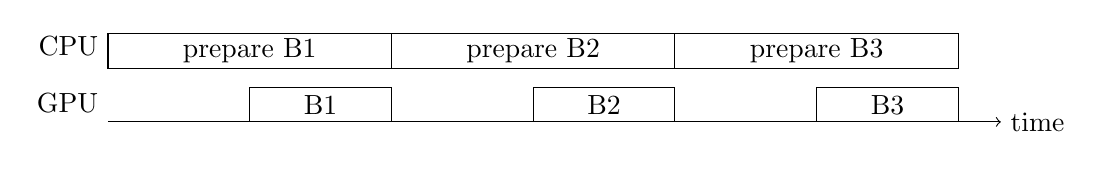
\begin{tikzpicture}[x=18mm,y=8mm]
\draw[->] (0,0) -- (6.3,0) node[right]{time};
\node[left] at (0,1.2) {CPU};
\node[left] at (0,0.3) {GPU};
\foreach \x/\lab in {0/B1,2/B2,4/B3} {
  \draw (\x,0.85) rectangle ++(2,0.55) node[midway]{prepare \lab};
}
\foreach \x/\lab in {1/B1,3/B2,5/B3} {
  \draw (\x,0.0) rectangle ++(1,0.55) node[midway]{\lab};
}
\end{tikzpicture}
\caption{Prefetching overlaps CPU preparation of batch \(n+1\) with GPU computation on batch \(n\).}
\label{fig:prefetching-overlap}
\end{figure}

Increasing workers helps only until another resource becomes limiting; the bottleneck may migrate from CPU decode to disk, network, memory bandwidth, host-to-device transfer, or finally model compute.

\subsection{Online inference}
Serving usually cares more about request latency and tail latency than raw samples/s.

\begin{figure}[htbp]
\centering
\begin{tikzpicture}[>=Latex, node distance=8mm and 11mm, every node/.style={draw, rounded corners, align=center, minimum height=8mm}]
\node (req) {request};
\node[right=of req] (api) {API / router};
\node[right=of api] (feature) {Redis /\\feature lookup};
\node[right=of feature] (queue) {batch /\\queue};
\node[right=of queue] (model) {model\\server};
\node[right=of model] (resp) {response};
\draw[->, thick] (req)--(api)--(feature)--(queue)--(model)--(resp);
\end{tikzpicture}
\caption{End-to-end serving latency contains infrastructure and data-access costs in addition to neural-network compute.}
\label{fig:inference-request-path}
\end{figure}

A useful decomposition is
\[
\underbrace{L_{\text{total}}}_{\text{request latency}}
\approx
\underbrace{L_{\text{network}}}_{\text{transport}}
+
\underbrace{L_{\text{lookup}}}_{\text{features / state}}
+
\underbrace{L_{\text{queue}}}_{\text{waiting}}
+
\underbrace{L_{\text{model}}}_{\text{inference}}
+
\underbrace{L_{\text{post}}}_{\text{post-processing}}.
\]
Optimising a 20 ms model is low leverage if another stage contributes 150 ms.

Tail metrics such as \(p_{95}\) and \(p_{99}\) expose rare slow requests hidden by a good mean.
\textbf{Dynamic batching} waits briefly to combine requests into a GPU-efficient batch, trading some per-request latency for higher accelerator throughput.

% BOOK-LINK: Link training throughput to batching/distributed training and serving latency to the inference chapter.


\section{Performance Arithmetic}
\label{sec:performance-arithmetic}
\label{sec:system-design-optimisation}
\label{sec:data-system-optionality}

Back-of-the-envelope arithmetic is often enough to identify an impossible architecture before profiling it.
If decoded samples have size \(D_s\), each batch contains \(B\) samples, and the accelerator consumes \(r_b\) batches/s, then
\[
\underbrace{\dot D_{\text{required}}}_{\text{required input bandwidth}}
=
\underbrace{D_s}_{\text{bytes / sample}}
\times
\underbrace{B}_{\text{samples / batch}}
\times
\underbrace{r_b}_{\text{batches / second}}.
\]
For \(D_s=2\) MB, \(B=256\), and \(r_b=4\), the data path must sustain roughly 2 GB/s after decoding.
A storage path supplying 0.5 GB/s cannot keep that workload fed regardless of model optimisation.


\begin{table}[htbp]
\centering
\caption{Qualitative tradeoffs of common layers.}
\label{tab:storage-tradeoffs}
\begin{tabularx}{\linewidth}{@{}lXXXX@{}}
\toprule
\textbf{Layer} & \textbf{Latency} & \textbf{Capacity} & \textbf{Durability} & \textbf{Natural role} \\
\midrule
GPU memory & extremely low & small & low & active tensors / model state \\
CPU RAM & low & moderate & low & working set / preprocessing \\
Local SSD & moderate & large & machine-local & dataset/cache staging \\
Redis & low network lookup & RAM-limited / sharded & configuration-dependent & hot shared state / cache \\
Relational DB & moderate & large & strong & structured canonical state \\
Object storage & high per-access & very large & high & durable datasets / checkpoints \\
\bottomrule
\end{tabularx}
\end{table}

Choosing a system based on the task:
\begin{itemize}
    \item Small experiment metadata on one machine \(\rightarrow\) files or SQLite.
    \item Concurrent structured state and flexible queries \(\rightarrow\) relational database.
    \item Repeated low-latency \(\text{entity ID}\rightarrow\text{feature}\) access \(\rightarrow\) Redis-like cache/key--value storage.
    \item Multi-terabyte or petabyte training corpora \(\rightarrow\) object storage plus sharded files.
    \item Semantic similarity search \(\rightarrow\) a vector index.
\end{itemize}

\section{Overview}
\label{sec:data-systems-evolution}
\label{sec:inductive-bias-data-systems}

\begin{table}[htbp]
\centering
\caption{Useful memory model: each component encodes an access-pattern bias.}
\label{tab:inductive-bias-data-systems}
\begin{tabularx}{\linewidth}{@{}lX@{}}
\toprule
\textbf{Technology} & \textbf{Structural assumption / inductive bias} \\
\midrule
Array & data is regularly indexed and numerical \\
Hash map & exact key identity is known \\
Tree index & ordering and range queries matter \\
Queue & producer and consumer rates should be decoupled \\
Relational DB & structured entities and relationships matter \\
Redis / cache & low-latency repeated key-based access matters \\
Parquet / columnar store & scans touch subsets of columns over many rows \\
Object store & large durable objects can be accessed remotely \\
Kafka-like log & data is an ordered replayable event stream \\
Vector index & semantic similarity maps to geometric proximity \\
Sharding & workload can be partitioned across machines \\
Replication & duplicate copies improve availability/read capacity \\
\bottomrule
\end{tabularx}
\end{table}


\begin{figure}[htbp]
\centering
\resizebox{0.88\linewidth}{!}{%
\begin{tikzpicture}[>=Latex, node distance=9mm and 22mm, every node/.style={align=center}]
\node[draw, diamond, aspect=2.1] (low) {GPU utilisation low?};
\node[draw, rounded corners, below left=of low] (compute) {No\\model/GPU compute may\\already dominate};
\node[draw, diamond, aspect=2.1, below right=of low] (wait) {GPU waiting\\for batches?};
\node[draw, rounded corners, below left=of wait] (other) {No\\profile kernels, synchronisation,\\communication};
\node[draw, rounded corners, below right=of wait] (path) {Yes\\profile storage $\rightarrow$ network $\rightarrow$\\CPU decode $\rightarrow$ queue $\rightarrow$ H2D};
\draw[->, thick] (low)--node[above left]{no}(compute);
\draw[->, thick] (low)--node[above right]{yes}(wait);
\draw[->, thick] (wait)--node[above left]{no}(other);
\draw[->, thick] (wait)--node[above right]{yes}(path);
\end{tikzpicture}%
}
\caption{A diagnostic tree for separating model-compute bottlenecks from input-pipeline bottlenecks.}
\label{fig:training-diagnostic-tree}
\end{figure}

A Redis-backed inference example follows the same reasoning: if requests repeatedly need \(\texttt{user\_id}\rightarrow\text{embedding}\), an in-memory shared cache matches the access pattern; when one node becomes too small, shard the keys; when node loss becomes unacceptable, replicate the shards; once copies exist, consistency and invalidation become explicit design problems.